\documentclass[12pt]{article}

\usepackage[utf8]{inputenc}
\usepackage[T1]{fontenc}
\usepackage[catalan]{babel}
\usepackage{lmodern}
\usepackage{geometry}
\usepackage{hyperref}
\usepackage{xcolor}
\usepackage[bf,sf,small,pagestyles]{titlesec}
\usepackage[font={footnotesize, sf}, labelfont=bf]{caption} 
\usepackage{siunitx}
\usepackage{graphicx}
\usepackage{booktabs}
\usepackage{amsmath,amssymb}
\usepackage{mathtools}
\usepackage[catalan,sort]{cleveref}

\geometry{
	a4paper,
	right = 2.5cm,
	left = 2.5cm,
	bottom = 3cm,
	top = 3cm
}

\hypersetup{
	colorlinks,
	linkcolor = {red!50!blue},
	linktoc = page
}

\crefname{figure}{figura}{figures}
\crefname{table}{taula}{taules}
\numberwithin{table}{section}
\numberwithin{figure}{section}
\numberwithin{equation}{section}

\graphicspath{{./figs/}}

% Unitats
\sisetup{
	inter-unit-product = \ensuremath{ \cdot },
	allow-number-unit-breaks = true,
	detect-family = true,
	list-final-separator = { i },
	list-units = single
}

\newcommand{\Z}{\mathbb{Z}}
\newcommand{\N}{\mathbb{N}}
\newcommand{\R}{\mathbb{R}}
\newcommand{\abs}[1]{\left\lvert #1 \right\rvert}
\DeclarePairedDelimiter{\ceil}{\lceil}{\rceil}
\newcommand{\parbreak}{
	\begin{center}
		--- $\ast$ ---
	\end{center} 
}
\makeatletter
\newcommand*{\defeq}{\mathrel{\rlap{%
    \raisebox{0.3ex}{$\m@th\cdot$}}%
  \raisebox{-0.3ex}{$\m@th\cdot$}}%
=}
\makeatother

\newpagestyle{pagina}{
	\headrule
	\sethead*{\sffamily {\bfseries Pràctica 3:} Interpolació polinòmica i integració numèrica}{}{\sffamily \sectiontitle}
	\footrule
	\setfoot*{}{}{\sffamily \thepage}
}
\renewpagestyle{plain}{
	\footrule
	\setfoot*{}{}{\sffamily \thepage}
}
\pagestyle{pagina}

\titleformat{\section}[hang]{\bfseries \sffamily \Large}{}{0pt}{}{\thispagestyle{plain}}

\title{\sffamily {\bfseries Pràctica 3:} Interpolació polinòmica i integració numèrica}
\author{\sffamily Arnau Mas}
\date{\sffamily 24 d'Abril 2018}

\begin{document}
\maketitle

\section{Problema 1} \label{sec:Problema 1}
L'objectiu d'aquest problema és interpolar la funció \( f \colon \R \to \R \) donada per
\begin{equation*}
	f(x) = \frac{1}{1 + 25x^2}
\end{equation*}
a l'interval \( [-1,1] \) mitjançant el polinomi interpolador de Lagrange. Es faran servir dos conjunts de nodes diferents per a realitzar la interpolació. En primer lloc, \( n \) nodes equidistants dins de l'interval, és a dir, donats per
\begin{equation*}
	x_k = -1 + \frac{2k}{n}
\end{equation*}
per \( k \in \{0, \cdots, n-1\} \). Els altres nodes que farem servir seran nodes de Chebyshev, definits com
\begin{equation*}
	x_k = \cos{\left(\frac{2k+1}{n+1} \frac{\pi}{2}\right)}
\end{equation*}
per \( k \in \{0, \cdots, n-1\} \). Es proposa fer la interpolació fent servir 4, 8, 16, 32 i 64 nodes. 

El programa \texttt{nodes.c} genera una llista amb \( n \) nodes equidistants o de Chebyshev. Aquesta llista serveix d'entrada per al programa \texttt{prob1.c}, que implementa el mètode de diferències dividides de Newton per a calcular els coeficients del polinomi interpolador de Lagrange per als nodes donats. A més avalua aquest polinomi aplicant la regla de Horner als 181 punts proposats i busca el màxim error comès. El fitxer \texttt{diferencies\_dividides.c} conté la implementació de funcions auxiliars per aquests programes, com el càlcul de diferències dividides fent ús de l'expressió recursiva així com una implementació de la regla de Horner per avaluar un polinomi. 

\parbreak

Per a tenir una idea del màxim error que es comet en cada cas hem avaluat tant la funció com el polinomi en un nombre elevat de punts. En particular en els punts donats per \( x_k = \num{-0.989} + k \cdot \num{0.011} \) per \( k \in \{0, \cdots, 180\} \), que són 181 punts repartits de forma equidistant a l'interval on estem interpolant. Si denotem per \( L_n \) el polinomi de Lagrange de grau \( n \) obtingut a partir dels nodes \( \{(x_0, f(x_0), \cdots , (x_n, f(x_n)) \} \) aleshores, per tot \( x \) de l'interval \( [a,b] \) on estem interpolant existeix \( \xi \in [a,b] \) tal que 
\begin{equation*}
	f(x) - L_n(x) = \frac{f^{(n+1)}(\xi)}{(n+1)!}\omega(x) 
\end{equation*}
on \( \omega = (x-x_0)\cdots(x-x_n) \). En particular podem fitar l'error en la interpolació com
\begin{equation*}
	\abs{f(x) - L_n(x)} \leqslant \frac{\max_{x \in [a,b]}\abs{f^{(n+1)}(x)}}{(n+1)!}\abs{\omega(x)}.
\end{equation*}
Observem que l'únic que depèn de la tria de nodes és el factor \( \omega(x) \). Els nodes de Chebyshev apareixen quan intentem minimitzar \( \omega(x) \). La interpolació que hem realitzat posa de manifest la importància de fer una bona tria de nodes: amb nodes equidistants, l'error màxim en \( [-1,1] \) no tendeix a zero quan \( n \to \infty \). Interpolant amb nodes de Chebyshev això no passa. A la \cref{fig:interpolacio} hi ha representats el resultat d'interpolar \( f \) amb nodes equidistants i de Chebyshev. Quan el nombre de nodes és baix no s'aprecien grans diferències entre les dues tries, i en els dos casos el màxim error es comet a \( x = 0 \) ---en cada gràfic hi ha representat en vermell el punt on es comet el màxim error---. Per a 16 i 32 nodes, però, fent la interpolació amb nodes equidistants, l'error als extrems de l'interval es dispara i arriba a ser superior a \( 600 \) per 32 nodes. En canvi, interpolant amb els nodes de Chebyshev el comportament és molt més estable i l'error màxim és manté sempre a \( x = 0 \). 

\begin{figure}[p]
	\centering
	\sffamily \footnotesize
	% GNUPLOT: LaTeX picture with Postscript
\begingroup
  \makeatletter
  \providecommand\color[2][]{%
    \GenericError{(gnuplot) \space\space\space\@spaces}{%
      Package color not loaded in conjunction with
      terminal option `colourtext'%
    }{See the gnuplot documentation for explanation.%
    }{Either use 'blacktext' in gnuplot or load the package
      color.sty in LaTeX.}%
    \renewcommand\color[2][]{}%
  }%
  \providecommand\includegraphics[2][]{%
    \GenericError{(gnuplot) \space\space\space\@spaces}{%
      Package graphicx or graphics not loaded%
    }{See the gnuplot documentation for explanation.%
    }{The gnuplot epslatex terminal needs graphicx.sty or graphics.sty.}%
    \renewcommand\includegraphics[2][]{}%
  }%
  \providecommand\rotatebox[2]{#2}%
  \@ifundefined{ifGPcolor}{%
    \newif\ifGPcolor
    \GPcolortrue
  }{}%
  \@ifundefined{ifGPblacktext}{%
    \newif\ifGPblacktext
    \GPblacktextfalse
  }{}%
  % define a \g@addto@macro without @ in the name:
  \let\gplgaddtomacro\g@addto@macro
  % define empty templates for all commands taking text:
  \gdef\gplbacktext{}%
  \gdef\gplfronttext{}%
  \makeatother
  \ifGPblacktext
    % no textcolor at all
    \def\colorrgb#1{}%
    \def\colorgray#1{}%
  \else
    % gray or color?
    \ifGPcolor
      \def\colorrgb#1{\color[rgb]{#1}}%
      \def\colorgray#1{\color[gray]{#1}}%
      \expandafter\def\csname LTw\endcsname{\color{white}}%
      \expandafter\def\csname LTb\endcsname{\color{black}}%
      \expandafter\def\csname LTa\endcsname{\color{black}}%
      \expandafter\def\csname LT0\endcsname{\color[rgb]{1,0,0}}%
      \expandafter\def\csname LT1\endcsname{\color[rgb]{0,1,0}}%
      \expandafter\def\csname LT2\endcsname{\color[rgb]{0,0,1}}%
      \expandafter\def\csname LT3\endcsname{\color[rgb]{1,0,1}}%
      \expandafter\def\csname LT4\endcsname{\color[rgb]{0,1,1}}%
      \expandafter\def\csname LT5\endcsname{\color[rgb]{1,1,0}}%
      \expandafter\def\csname LT6\endcsname{\color[rgb]{0,0,0}}%
      \expandafter\def\csname LT7\endcsname{\color[rgb]{1,0.3,0}}%
      \expandafter\def\csname LT8\endcsname{\color[rgb]{0.5,0.5,0.5}}%
    \else
      % gray
      \def\colorrgb#1{\color{black}}%
      \def\colorgray#1{\color[gray]{#1}}%
      \expandafter\def\csname LTw\endcsname{\color{white}}%
      \expandafter\def\csname LTb\endcsname{\color{black}}%
      \expandafter\def\csname LTa\endcsname{\color{black}}%
      \expandafter\def\csname LT0\endcsname{\color{black}}%
      \expandafter\def\csname LT1\endcsname{\color{black}}%
      \expandafter\def\csname LT2\endcsname{\color{black}}%
      \expandafter\def\csname LT3\endcsname{\color{black}}%
      \expandafter\def\csname LT4\endcsname{\color{black}}%
      \expandafter\def\csname LT5\endcsname{\color{black}}%
      \expandafter\def\csname LT6\endcsname{\color{black}}%
      \expandafter\def\csname LT7\endcsname{\color{black}}%
      \expandafter\def\csname LT8\endcsname{\color{black}}%
    \fi
  \fi
    \setlength{\unitlength}{0.0500bp}%
    \ifx\gptboxheight\undefined%
      \newlength{\gptboxheight}%
      \newlength{\gptboxwidth}%
      \newsavebox{\gptboxtext}%
    \fi%
    \setlength{\fboxrule}{0.5pt}%
    \setlength{\fboxsep}{1pt}%
\begin{picture}(4534.00,2834.00)%
    \gplgaddtomacro\gplbacktext{%
      \csname LTb\endcsname%%
      \put(990,499){\makebox(0,0)[r]{\strut{}\num{-0.25}}}%
      \put(990,842){\makebox(0,0)[r]{\strut{}\num{0}}}%
      \put(990,1184){\makebox(0,0)[r]{\strut{}\num{0.25}}}%
      \put(990,1527){\makebox(0,0)[r]{\strut{}\num{0.5}}}%
      \put(990,1869){\makebox(0,0)[r]{\strut{}\num{0.75}}}%
      \put(990,2212){\makebox(0,0)[r]{\strut{}\num{1}}}%
      \put(990,2554){\makebox(0,0)[r]{\strut{}\num{1.25}}}%
      \put(1259,279){\makebox(0,0){\strut{}\num{-1}}}%
      \put(1944,279){\makebox(0,0){\strut{}\num{-0.5}}}%
      \put(2630,279){\makebox(0,0){\strut{}\num{0}}}%
      \put(3315,279){\makebox(0,0){\strut{}\num{0.5}}}%
      \put(4000,279){\makebox(0,0){\strut{}\num{1}}}%
      \put(2355,855){\makebox(0,0)[l]{\strut{}$ n = 4 $}}%
    }%
    \gplgaddtomacro\gplfronttext{%
    }%
    \gplbacktext
    \put(0,0){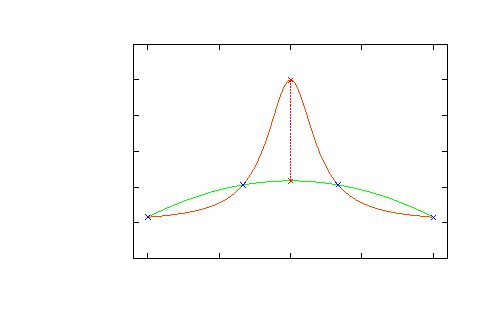
\includegraphics{04-eq}}%
    \gplfronttext
  \end{picture}%
\endgroup
% GNUPLOT: LaTeX picture with Postscript
\begingroup
  \makeatletter
  \providecommand\color[2][]{%
    \GenericError{(gnuplot) \space\space\space\@spaces}{%
      Package color not loaded in conjunction with
      terminal option `colourtext'%
    }{See the gnuplot documentation for explanation.%
    }{Either use 'blacktext' in gnuplot or load the package
      color.sty in LaTeX.}%
    \renewcommand\color[2][]{}%
  }%
  \providecommand\includegraphics[2][]{%
    \GenericError{(gnuplot) \space\space\space\@spaces}{%
      Package graphicx or graphics not loaded%
    }{See the gnuplot documentation for explanation.%
    }{The gnuplot epslatex terminal needs graphicx.sty or graphics.sty.}%
    \renewcommand\includegraphics[2][]{}%
  }%
  \providecommand\rotatebox[2]{#2}%
  \@ifundefined{ifGPcolor}{%
    \newif\ifGPcolor
    \GPcolortrue
  }{}%
  \@ifundefined{ifGPblacktext}{%
    \newif\ifGPblacktext
    \GPblacktextfalse
  }{}%
  % define a \g@addto@macro without @ in the name:
  \let\gplgaddtomacro\g@addto@macro
  % define empty templates for all commands taking text:
  \gdef\gplbacktext{}%
  \gdef\gplfronttext{}%
  \makeatother
  \ifGPblacktext
    % no textcolor at all
    \def\colorrgb#1{}%
    \def\colorgray#1{}%
  \else
    % gray or color?
    \ifGPcolor
      \def\colorrgb#1{\color[rgb]{#1}}%
      \def\colorgray#1{\color[gray]{#1}}%
      \expandafter\def\csname LTw\endcsname{\color{white}}%
      \expandafter\def\csname LTb\endcsname{\color{black}}%
      \expandafter\def\csname LTa\endcsname{\color{black}}%
      \expandafter\def\csname LT0\endcsname{\color[rgb]{1,0,0}}%
      \expandafter\def\csname LT1\endcsname{\color[rgb]{0,1,0}}%
      \expandafter\def\csname LT2\endcsname{\color[rgb]{0,0,1}}%
      \expandafter\def\csname LT3\endcsname{\color[rgb]{1,0,1}}%
      \expandafter\def\csname LT4\endcsname{\color[rgb]{0,1,1}}%
      \expandafter\def\csname LT5\endcsname{\color[rgb]{1,1,0}}%
      \expandafter\def\csname LT6\endcsname{\color[rgb]{0,0,0}}%
      \expandafter\def\csname LT7\endcsname{\color[rgb]{1,0.3,0}}%
      \expandafter\def\csname LT8\endcsname{\color[rgb]{0.5,0.5,0.5}}%
    \else
      % gray
      \def\colorrgb#1{\color{black}}%
      \def\colorgray#1{\color[gray]{#1}}%
      \expandafter\def\csname LTw\endcsname{\color{white}}%
      \expandafter\def\csname LTb\endcsname{\color{black}}%
      \expandafter\def\csname LTa\endcsname{\color{black}}%
      \expandafter\def\csname LT0\endcsname{\color{black}}%
      \expandafter\def\csname LT1\endcsname{\color{black}}%
      \expandafter\def\csname LT2\endcsname{\color{black}}%
      \expandafter\def\csname LT3\endcsname{\color{black}}%
      \expandafter\def\csname LT4\endcsname{\color{black}}%
      \expandafter\def\csname LT5\endcsname{\color{black}}%
      \expandafter\def\csname LT6\endcsname{\color{black}}%
      \expandafter\def\csname LT7\endcsname{\color{black}}%
      \expandafter\def\csname LT8\endcsname{\color{black}}%
    \fi
  \fi
    \setlength{\unitlength}{0.0500bp}%
    \ifx\gptboxheight\undefined%
      \newlength{\gptboxheight}%
      \newlength{\gptboxwidth}%
      \newsavebox{\gptboxtext}%
    \fi%
    \setlength{\fboxrule}{0.5pt}%
    \setlength{\fboxsep}{1pt}%
\begin{picture}(4534.00,2834.00)%
    \gplgaddtomacro\gplbacktext{%
      \csname LTb\endcsname%%
      \put(990,499){\makebox(0,0)[r]{\strut{}\num{-0.25}}}%
      \put(990,842){\makebox(0,0)[r]{\strut{}\num{0}}}%
      \put(990,1184){\makebox(0,0)[r]{\strut{}\num{0.25}}}%
      \put(990,1527){\makebox(0,0)[r]{\strut{}\num{0.5}}}%
      \put(990,1869){\makebox(0,0)[r]{\strut{}\num{0.75}}}%
      \put(990,2212){\makebox(0,0)[r]{\strut{}\num{1}}}%
      \put(990,2554){\makebox(0,0)[r]{\strut{}\num{1.25}}}%
      \put(1259,279){\makebox(0,0){\strut{}\num{-1}}}%
      \put(1944,279){\makebox(0,0){\strut{}\num{-0.5}}}%
      \put(2630,279){\makebox(0,0){\strut{}\num{0}}}%
      \put(3315,279){\makebox(0,0){\strut{}\num{0.5}}}%
      \put(4000,279){\makebox(0,0){\strut{}\num{1}}}%
      \put(2355,855){\makebox(0,0)[l]{\strut{}$ n = 4 $}}%
    }%
    \gplgaddtomacro\gplfronttext{%
    }%
    \gplbacktext
    \put(0,0){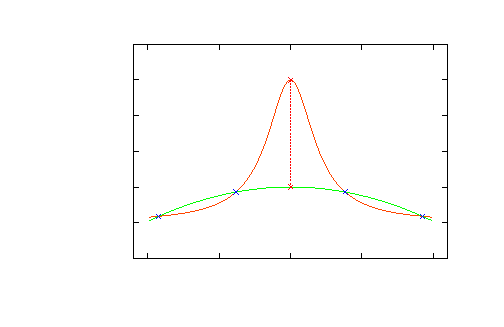
\includegraphics{04-cheb}}%
    \gplfronttext
  \end{picture}%
\endgroup

	% GNUPLOT: LaTeX picture with Postscript
\begingroup
  \makeatletter
  \providecommand\color[2][]{%
    \GenericError{(gnuplot) \space\space\space\@spaces}{%
      Package color not loaded in conjunction with
      terminal option `colourtext'%
    }{See the gnuplot documentation for explanation.%
    }{Either use 'blacktext' in gnuplot or load the package
      color.sty in LaTeX.}%
    \renewcommand\color[2][]{}%
  }%
  \providecommand\includegraphics[2][]{%
    \GenericError{(gnuplot) \space\space\space\@spaces}{%
      Package graphicx or graphics not loaded%
    }{See the gnuplot documentation for explanation.%
    }{The gnuplot epslatex terminal needs graphicx.sty or graphics.sty.}%
    \renewcommand\includegraphics[2][]{}%
  }%
  \providecommand\rotatebox[2]{#2}%
  \@ifundefined{ifGPcolor}{%
    \newif\ifGPcolor
    \GPcolortrue
  }{}%
  \@ifundefined{ifGPblacktext}{%
    \newif\ifGPblacktext
    \GPblacktextfalse
  }{}%
  % define a \g@addto@macro without @ in the name:
  \let\gplgaddtomacro\g@addto@macro
  % define empty templates for all commands taking text:
  \gdef\gplbacktext{}%
  \gdef\gplfronttext{}%
  \makeatother
  \ifGPblacktext
    % no textcolor at all
    \def\colorrgb#1{}%
    \def\colorgray#1{}%
  \else
    % gray or color?
    \ifGPcolor
      \def\colorrgb#1{\color[rgb]{#1}}%
      \def\colorgray#1{\color[gray]{#1}}%
      \expandafter\def\csname LTw\endcsname{\color{white}}%
      \expandafter\def\csname LTb\endcsname{\color{black}}%
      \expandafter\def\csname LTa\endcsname{\color{black}}%
      \expandafter\def\csname LT0\endcsname{\color[rgb]{1,0,0}}%
      \expandafter\def\csname LT1\endcsname{\color[rgb]{0,1,0}}%
      \expandafter\def\csname LT2\endcsname{\color[rgb]{0,0,1}}%
      \expandafter\def\csname LT3\endcsname{\color[rgb]{1,0,1}}%
      \expandafter\def\csname LT4\endcsname{\color[rgb]{0,1,1}}%
      \expandafter\def\csname LT5\endcsname{\color[rgb]{1,1,0}}%
      \expandafter\def\csname LT6\endcsname{\color[rgb]{0,0,0}}%
      \expandafter\def\csname LT7\endcsname{\color[rgb]{1,0.3,0}}%
      \expandafter\def\csname LT8\endcsname{\color[rgb]{0.5,0.5,0.5}}%
    \else
      % gray
      \def\colorrgb#1{\color{black}}%
      \def\colorgray#1{\color[gray]{#1}}%
      \expandafter\def\csname LTw\endcsname{\color{white}}%
      \expandafter\def\csname LTb\endcsname{\color{black}}%
      \expandafter\def\csname LTa\endcsname{\color{black}}%
      \expandafter\def\csname LT0\endcsname{\color{black}}%
      \expandafter\def\csname LT1\endcsname{\color{black}}%
      \expandafter\def\csname LT2\endcsname{\color{black}}%
      \expandafter\def\csname LT3\endcsname{\color{black}}%
      \expandafter\def\csname LT4\endcsname{\color{black}}%
      \expandafter\def\csname LT5\endcsname{\color{black}}%
      \expandafter\def\csname LT6\endcsname{\color{black}}%
      \expandafter\def\csname LT7\endcsname{\color{black}}%
      \expandafter\def\csname LT8\endcsname{\color{black}}%
    \fi
  \fi
    \setlength{\unitlength}{0.0500bp}%
    \ifx\gptboxheight\undefined%
      \newlength{\gptboxheight}%
      \newlength{\gptboxwidth}%
      \newsavebox{\gptboxtext}%
    \fi%
    \setlength{\fboxrule}{0.5pt}%
    \setlength{\fboxsep}{1pt}%
\begin{picture}(3968.00,3968.00)%
    \gplgaddtomacro\gplbacktext{%
      \csname LTb\endcsname%%
      \put(726,440){\makebox(0,0)[r]{\strut{}\num{0}}}%
      \put(726,991){\makebox(0,0)[r]{\strut{}\num{0.2}}}%
      \put(726,1542){\makebox(0,0)[r]{\strut{}\num{0.4}}}%
      \put(726,2094){\makebox(0,0)[r]{\strut{}\num{0.6}}}%
      \put(726,2645){\makebox(0,0)[r]{\strut{}\num{0.8}}}%
      \put(726,3196){\makebox(0,0)[r]{\strut{}\num{1}}}%
      \put(726,3747){\makebox(0,0)[r]{\strut{}\num{1.2}}}%
      \put(981,220){\makebox(0,0){\strut{}\num{-1}}}%
      \put(1598,220){\makebox(0,0){\strut{}\num{-0.5}}}%
      \put(2215,220){\makebox(0,0){\strut{}\num{0}}}%
      \put(2831,220){\makebox(0,0){\strut{}\num{0.5}}}%
      \put(3448,220){\makebox(0,0){\strut{}\num{1}}}%
    }%
    \gplgaddtomacro\gplfronttext{%
    }%
    \gplbacktext
    \put(0,0){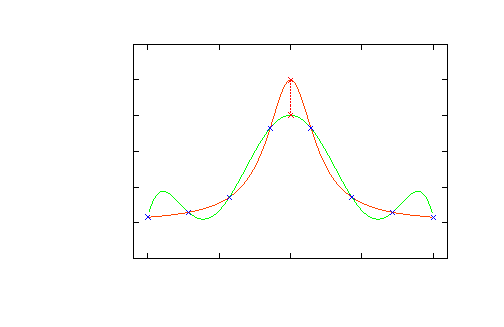
\includegraphics{08-eq}}%
    \gplfronttext
  \end{picture}%
\endgroup
% GNUPLOT: LaTeX picture with Postscript
\begingroup
  \makeatletter
  \providecommand\color[2][]{%
    \GenericError{(gnuplot) \space\space\space\@spaces}{%
      Package color not loaded in conjunction with
      terminal option `colourtext'%
    }{See the gnuplot documentation for explanation.%
    }{Either use 'blacktext' in gnuplot or load the package
      color.sty in LaTeX.}%
    \renewcommand\color[2][]{}%
  }%
  \providecommand\includegraphics[2][]{%
    \GenericError{(gnuplot) \space\space\space\@spaces}{%
      Package graphicx or graphics not loaded%
    }{See the gnuplot documentation for explanation.%
    }{The gnuplot epslatex terminal needs graphicx.sty or graphics.sty.}%
    \renewcommand\includegraphics[2][]{}%
  }%
  \providecommand\rotatebox[2]{#2}%
  \@ifundefined{ifGPcolor}{%
    \newif\ifGPcolor
    \GPcolortrue
  }{}%
  \@ifundefined{ifGPblacktext}{%
    \newif\ifGPblacktext
    \GPblacktextfalse
  }{}%
  % define a \g@addto@macro without @ in the name:
  \let\gplgaddtomacro\g@addto@macro
  % define empty templates for all commands taking text:
  \gdef\gplbacktext{}%
  \gdef\gplfronttext{}%
  \makeatother
  \ifGPblacktext
    % no textcolor at all
    \def\colorrgb#1{}%
    \def\colorgray#1{}%
  \else
    % gray or color?
    \ifGPcolor
      \def\colorrgb#1{\color[rgb]{#1}}%
      \def\colorgray#1{\color[gray]{#1}}%
      \expandafter\def\csname LTw\endcsname{\color{white}}%
      \expandafter\def\csname LTb\endcsname{\color{black}}%
      \expandafter\def\csname LTa\endcsname{\color{black}}%
      \expandafter\def\csname LT0\endcsname{\color[rgb]{1,0,0}}%
      \expandafter\def\csname LT1\endcsname{\color[rgb]{0,1,0}}%
      \expandafter\def\csname LT2\endcsname{\color[rgb]{0,0,1}}%
      \expandafter\def\csname LT3\endcsname{\color[rgb]{1,0,1}}%
      \expandafter\def\csname LT4\endcsname{\color[rgb]{0,1,1}}%
      \expandafter\def\csname LT5\endcsname{\color[rgb]{1,1,0}}%
      \expandafter\def\csname LT6\endcsname{\color[rgb]{0,0,0}}%
      \expandafter\def\csname LT7\endcsname{\color[rgb]{1,0.3,0}}%
      \expandafter\def\csname LT8\endcsname{\color[rgb]{0.5,0.5,0.5}}%
    \else
      % gray
      \def\colorrgb#1{\color{black}}%
      \def\colorgray#1{\color[gray]{#1}}%
      \expandafter\def\csname LTw\endcsname{\color{white}}%
      \expandafter\def\csname LTb\endcsname{\color{black}}%
      \expandafter\def\csname LTa\endcsname{\color{black}}%
      \expandafter\def\csname LT0\endcsname{\color{black}}%
      \expandafter\def\csname LT1\endcsname{\color{black}}%
      \expandafter\def\csname LT2\endcsname{\color{black}}%
      \expandafter\def\csname LT3\endcsname{\color{black}}%
      \expandafter\def\csname LT4\endcsname{\color{black}}%
      \expandafter\def\csname LT5\endcsname{\color{black}}%
      \expandafter\def\csname LT6\endcsname{\color{black}}%
      \expandafter\def\csname LT7\endcsname{\color{black}}%
      \expandafter\def\csname LT8\endcsname{\color{black}}%
    \fi
  \fi
    \setlength{\unitlength}{0.0500bp}%
    \ifx\gptboxheight\undefined%
      \newlength{\gptboxheight}%
      \newlength{\gptboxwidth}%
      \newsavebox{\gptboxtext}%
    \fi%
    \setlength{\fboxrule}{0.5pt}%
    \setlength{\fboxsep}{1pt}%
\begin{picture}(3968.00,3968.00)%
    \gplgaddtomacro\gplbacktext{%
      \csname LTb\endcsname%%
      \put(726,440){\makebox(0,0)[r]{\strut{}\num{0}}}%
      \put(726,991){\makebox(0,0)[r]{\strut{}\num{0.2}}}%
      \put(726,1542){\makebox(0,0)[r]{\strut{}\num{0.4}}}%
      \put(726,2094){\makebox(0,0)[r]{\strut{}\num{0.6}}}%
      \put(726,2645){\makebox(0,0)[r]{\strut{}\num{0.8}}}%
      \put(726,3196){\makebox(0,0)[r]{\strut{}\num{1}}}%
      \put(726,3747){\makebox(0,0)[r]{\strut{}\num{1.2}}}%
      \put(981,220){\makebox(0,0){\strut{}\num{-1}}}%
      \put(1598,220){\makebox(0,0){\strut{}\num{-0.5}}}%
      \put(2215,220){\makebox(0,0){\strut{}\num{0}}}%
      \put(2831,220){\makebox(0,0){\strut{}\num{0.5}}}%
      \put(3448,220){\makebox(0,0){\strut{}\num{1}}}%
    }%
    \gplgaddtomacro\gplfronttext{%
    }%
    \gplbacktext
    \put(0,0){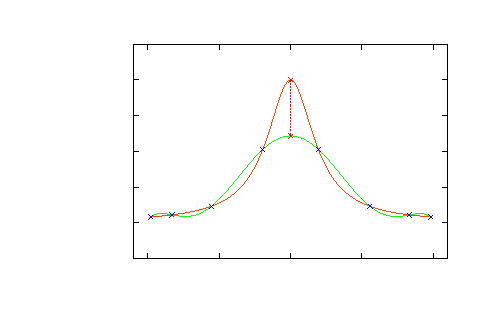
\includegraphics{08-cheb}}%
    \gplfronttext
  \end{picture}%
\endgroup

	% GNUPLOT: LaTeX picture with Postscript
\begingroup
  \makeatletter
  \providecommand\color[2][]{%
    \GenericError{(gnuplot) \space\space\space\@spaces}{%
      Package color not loaded in conjunction with
      terminal option `colourtext'%
    }{See the gnuplot documentation for explanation.%
    }{Either use 'blacktext' in gnuplot or load the package
      color.sty in LaTeX.}%
    \renewcommand\color[2][]{}%
  }%
  \providecommand\includegraphics[2][]{%
    \GenericError{(gnuplot) \space\space\space\@spaces}{%
      Package graphicx or graphics not loaded%
    }{See the gnuplot documentation for explanation.%
    }{The gnuplot epslatex terminal needs graphicx.sty or graphics.sty.}%
    \renewcommand\includegraphics[2][]{}%
  }%
  \providecommand\rotatebox[2]{#2}%
  \@ifundefined{ifGPcolor}{%
    \newif\ifGPcolor
    \GPcolortrue
  }{}%
  \@ifundefined{ifGPblacktext}{%
    \newif\ifGPblacktext
    \GPblacktextfalse
  }{}%
  % define a \g@addto@macro without @ in the name:
  \let\gplgaddtomacro\g@addto@macro
  % define empty templates for all commands taking text:
  \gdef\gplbacktext{}%
  \gdef\gplfronttext{}%
  \makeatother
  \ifGPblacktext
    % no textcolor at all
    \def\colorrgb#1{}%
    \def\colorgray#1{}%
  \else
    % gray or color?
    \ifGPcolor
      \def\colorrgb#1{\color[rgb]{#1}}%
      \def\colorgray#1{\color[gray]{#1}}%
      \expandafter\def\csname LTw\endcsname{\color{white}}%
      \expandafter\def\csname LTb\endcsname{\color{black}}%
      \expandafter\def\csname LTa\endcsname{\color{black}}%
      \expandafter\def\csname LT0\endcsname{\color[rgb]{1,0,0}}%
      \expandafter\def\csname LT1\endcsname{\color[rgb]{0,1,0}}%
      \expandafter\def\csname LT2\endcsname{\color[rgb]{0,0,1}}%
      \expandafter\def\csname LT3\endcsname{\color[rgb]{1,0,1}}%
      \expandafter\def\csname LT4\endcsname{\color[rgb]{0,1,1}}%
      \expandafter\def\csname LT5\endcsname{\color[rgb]{1,1,0}}%
      \expandafter\def\csname LT6\endcsname{\color[rgb]{0,0,0}}%
      \expandafter\def\csname LT7\endcsname{\color[rgb]{1,0.3,0}}%
      \expandafter\def\csname LT8\endcsname{\color[rgb]{0.5,0.5,0.5}}%
    \else
      % gray
      \def\colorrgb#1{\color{black}}%
      \def\colorgray#1{\color[gray]{#1}}%
      \expandafter\def\csname LTw\endcsname{\color{white}}%
      \expandafter\def\csname LTb\endcsname{\color{black}}%
      \expandafter\def\csname LTa\endcsname{\color{black}}%
      \expandafter\def\csname LT0\endcsname{\color{black}}%
      \expandafter\def\csname LT1\endcsname{\color{black}}%
      \expandafter\def\csname LT2\endcsname{\color{black}}%
      \expandafter\def\csname LT3\endcsname{\color{black}}%
      \expandafter\def\csname LT4\endcsname{\color{black}}%
      \expandafter\def\csname LT5\endcsname{\color{black}}%
      \expandafter\def\csname LT6\endcsname{\color{black}}%
      \expandafter\def\csname LT7\endcsname{\color{black}}%
      \expandafter\def\csname LT8\endcsname{\color{black}}%
    \fi
  \fi
    \setlength{\unitlength}{0.0500bp}%
    \ifx\gptboxheight\undefined%
      \newlength{\gptboxheight}%
      \newlength{\gptboxwidth}%
      \newsavebox{\gptboxtext}%
    \fi%
    \setlength{\fboxrule}{0.5pt}%
    \setlength{\fboxsep}{1pt}%
\begin{picture}(4534.00,2834.00)%
    \gplgaddtomacro\gplbacktext{%
      \csname LTb\endcsname%%
      \put(990,499){\makebox(0,0)[r]{\strut{}\num{-0.25}}}%
      \put(990,842){\makebox(0,0)[r]{\strut{}\num{0}}}%
      \put(990,1184){\makebox(0,0)[r]{\strut{}\num{0.25}}}%
      \put(990,1527){\makebox(0,0)[r]{\strut{}\num{0.5}}}%
      \put(990,1869){\makebox(0,0)[r]{\strut{}\num{0.75}}}%
      \put(990,2212){\makebox(0,0)[r]{\strut{}\num{1}}}%
      \put(990,2554){\makebox(0,0)[r]{\strut{}\num{1.25}}}%
      \put(1259,279){\makebox(0,0){\strut{}\num{-1}}}%
      \put(1944,279){\makebox(0,0){\strut{}\num{-0.5}}}%
      \put(2630,279){\makebox(0,0){\strut{}\num{0}}}%
      \put(3315,279){\makebox(0,0){\strut{}\num{0.5}}}%
      \put(4000,279){\makebox(0,0){\strut{}\num{1}}}%
      \put(2355,855){\makebox(0,0)[l]{\strut{}$ n = 16 $}}%
      \put(2355,855){\makebox(0,0)[l]{\strut{}$ n = 16 $}}%
    }%
    \gplgaddtomacro\gplfronttext{%
    }%
    \gplbacktext
    \put(0,0){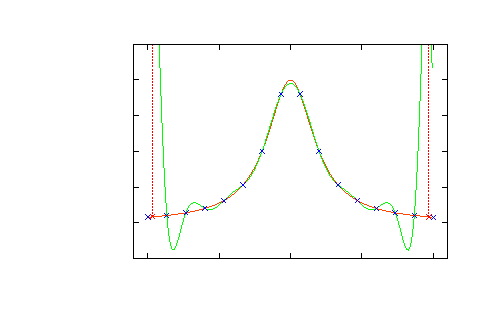
\includegraphics{16-eq}}%
    \gplfronttext
  \end{picture}%
\endgroup
% GNUPLOT: LaTeX picture with Postscript
\begingroup
  \makeatletter
  \providecommand\color[2][]{%
    \GenericError{(gnuplot) \space\space\space\@spaces}{%
      Package color not loaded in conjunction with
      terminal option `colourtext'%
    }{See the gnuplot documentation for explanation.%
    }{Either use 'blacktext' in gnuplot or load the package
      color.sty in LaTeX.}%
    \renewcommand\color[2][]{}%
  }%
  \providecommand\includegraphics[2][]{%
    \GenericError{(gnuplot) \space\space\space\@spaces}{%
      Package graphicx or graphics not loaded%
    }{See the gnuplot documentation for explanation.%
    }{The gnuplot epslatex terminal needs graphicx.sty or graphics.sty.}%
    \renewcommand\includegraphics[2][]{}%
  }%
  \providecommand\rotatebox[2]{#2}%
  \@ifundefined{ifGPcolor}{%
    \newif\ifGPcolor
    \GPcolortrue
  }{}%
  \@ifundefined{ifGPblacktext}{%
    \newif\ifGPblacktext
    \GPblacktextfalse
  }{}%
  % define a \g@addto@macro without @ in the name:
  \let\gplgaddtomacro\g@addto@macro
  % define empty templates for all commands taking text:
  \gdef\gplbacktext{}%
  \gdef\gplfronttext{}%
  \makeatother
  \ifGPblacktext
    % no textcolor at all
    \def\colorrgb#1{}%
    \def\colorgray#1{}%
  \else
    % gray or color?
    \ifGPcolor
      \def\colorrgb#1{\color[rgb]{#1}}%
      \def\colorgray#1{\color[gray]{#1}}%
      \expandafter\def\csname LTw\endcsname{\color{white}}%
      \expandafter\def\csname LTb\endcsname{\color{black}}%
      \expandafter\def\csname LTa\endcsname{\color{black}}%
      \expandafter\def\csname LT0\endcsname{\color[rgb]{1,0,0}}%
      \expandafter\def\csname LT1\endcsname{\color[rgb]{0,1,0}}%
      \expandafter\def\csname LT2\endcsname{\color[rgb]{0,0,1}}%
      \expandafter\def\csname LT3\endcsname{\color[rgb]{1,0,1}}%
      \expandafter\def\csname LT4\endcsname{\color[rgb]{0,1,1}}%
      \expandafter\def\csname LT5\endcsname{\color[rgb]{1,1,0}}%
      \expandafter\def\csname LT6\endcsname{\color[rgb]{0,0,0}}%
      \expandafter\def\csname LT7\endcsname{\color[rgb]{1,0.3,0}}%
      \expandafter\def\csname LT8\endcsname{\color[rgb]{0.5,0.5,0.5}}%
    \else
      % gray
      \def\colorrgb#1{\color{black}}%
      \def\colorgray#1{\color[gray]{#1}}%
      \expandafter\def\csname LTw\endcsname{\color{white}}%
      \expandafter\def\csname LTb\endcsname{\color{black}}%
      \expandafter\def\csname LTa\endcsname{\color{black}}%
      \expandafter\def\csname LT0\endcsname{\color{black}}%
      \expandafter\def\csname LT1\endcsname{\color{black}}%
      \expandafter\def\csname LT2\endcsname{\color{black}}%
      \expandafter\def\csname LT3\endcsname{\color{black}}%
      \expandafter\def\csname LT4\endcsname{\color{black}}%
      \expandafter\def\csname LT5\endcsname{\color{black}}%
      \expandafter\def\csname LT6\endcsname{\color{black}}%
      \expandafter\def\csname LT7\endcsname{\color{black}}%
      \expandafter\def\csname LT8\endcsname{\color{black}}%
    \fi
  \fi
    \setlength{\unitlength}{0.0500bp}%
    \ifx\gptboxheight\undefined%
      \newlength{\gptboxheight}%
      \newlength{\gptboxwidth}%
      \newsavebox{\gptboxtext}%
    \fi%
    \setlength{\fboxrule}{0.5pt}%
    \setlength{\fboxsep}{1pt}%
\begin{picture}(4534.00,4534.00)%
    \gplgaddtomacro\gplbacktext{%
      \csname LTb\endcsname%%
      \put(990,1349){\makebox(0,0)[r]{\strut{}\num{-0.25}}}%
      \put(990,1692){\makebox(0,0)[r]{\strut{}\num{0}}}%
      \put(990,2034){\makebox(0,0)[r]{\strut{}\num{0.25}}}%
      \put(990,2377){\makebox(0,0)[r]{\strut{}\num{0.5}}}%
      \put(990,2719){\makebox(0,0)[r]{\strut{}\num{0.75}}}%
      \put(990,3062){\makebox(0,0)[r]{\strut{}\num{1}}}%
      \put(990,3404){\makebox(0,0)[r]{\strut{}\num{1.25}}}%
      \put(1259,1129){\makebox(0,0){\strut{}\num{-1}}}%
      \put(1944,1129){\makebox(0,0){\strut{}\num{-0.5}}}%
      \put(2630,1129){\makebox(0,0){\strut{}\num{0}}}%
      \put(3315,1129){\makebox(0,0){\strut{}\num{0.5}}}%
      \put(4000,1129){\makebox(0,0){\strut{}\num{1}}}%
    }%
    \gplgaddtomacro\gplfronttext{%
    }%
    \gplbacktext
    \put(0,0){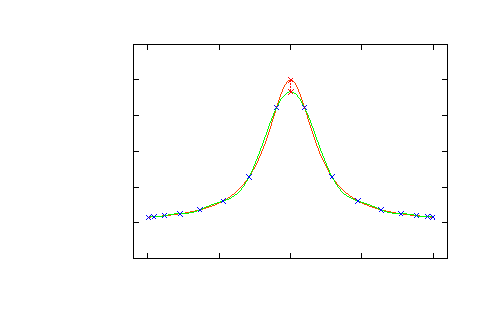
\includegraphics{16-cheb}}%
    \gplfronttext
  \end{picture}%
\endgroup

	% GNUPLOT: LaTeX picture with Postscript
\begingroup
  \makeatletter
  \providecommand\color[2][]{%
    \GenericError{(gnuplot) \space\space\space\@spaces}{%
      Package color not loaded in conjunction with
      terminal option `colourtext'%
    }{See the gnuplot documentation for explanation.%
    }{Either use 'blacktext' in gnuplot or load the package
      color.sty in LaTeX.}%
    \renewcommand\color[2][]{}%
  }%
  \providecommand\includegraphics[2][]{%
    \GenericError{(gnuplot) \space\space\space\@spaces}{%
      Package graphicx or graphics not loaded%
    }{See the gnuplot documentation for explanation.%
    }{The gnuplot epslatex terminal needs graphicx.sty or graphics.sty.}%
    \renewcommand\includegraphics[2][]{}%
  }%
  \providecommand\rotatebox[2]{#2}%
  \@ifundefined{ifGPcolor}{%
    \newif\ifGPcolor
    \GPcolortrue
  }{}%
  \@ifundefined{ifGPblacktext}{%
    \newif\ifGPblacktext
    \GPblacktextfalse
  }{}%
  % define a \g@addto@macro without @ in the name:
  \let\gplgaddtomacro\g@addto@macro
  % define empty templates for all commands taking text:
  \gdef\gplbacktext{}%
  \gdef\gplfronttext{}%
  \makeatother
  \ifGPblacktext
    % no textcolor at all
    \def\colorrgb#1{}%
    \def\colorgray#1{}%
  \else
    % gray or color?
    \ifGPcolor
      \def\colorrgb#1{\color[rgb]{#1}}%
      \def\colorgray#1{\color[gray]{#1}}%
      \expandafter\def\csname LTw\endcsname{\color{white}}%
      \expandafter\def\csname LTb\endcsname{\color{black}}%
      \expandafter\def\csname LTa\endcsname{\color{black}}%
      \expandafter\def\csname LT0\endcsname{\color[rgb]{1,0,0}}%
      \expandafter\def\csname LT1\endcsname{\color[rgb]{0,1,0}}%
      \expandafter\def\csname LT2\endcsname{\color[rgb]{0,0,1}}%
      \expandafter\def\csname LT3\endcsname{\color[rgb]{1,0,1}}%
      \expandafter\def\csname LT4\endcsname{\color[rgb]{0,1,1}}%
      \expandafter\def\csname LT5\endcsname{\color[rgb]{1,1,0}}%
      \expandafter\def\csname LT6\endcsname{\color[rgb]{0,0,0}}%
      \expandafter\def\csname LT7\endcsname{\color[rgb]{1,0.3,0}}%
      \expandafter\def\csname LT8\endcsname{\color[rgb]{0.5,0.5,0.5}}%
    \else
      % gray
      \def\colorrgb#1{\color{black}}%
      \def\colorgray#1{\color[gray]{#1}}%
      \expandafter\def\csname LTw\endcsname{\color{white}}%
      \expandafter\def\csname LTb\endcsname{\color{black}}%
      \expandafter\def\csname LTa\endcsname{\color{black}}%
      \expandafter\def\csname LT0\endcsname{\color{black}}%
      \expandafter\def\csname LT1\endcsname{\color{black}}%
      \expandafter\def\csname LT2\endcsname{\color{black}}%
      \expandafter\def\csname LT3\endcsname{\color{black}}%
      \expandafter\def\csname LT4\endcsname{\color{black}}%
      \expandafter\def\csname LT5\endcsname{\color{black}}%
      \expandafter\def\csname LT6\endcsname{\color{black}}%
      \expandafter\def\csname LT7\endcsname{\color{black}}%
      \expandafter\def\csname LT8\endcsname{\color{black}}%
    \fi
  \fi
    \setlength{\unitlength}{0.0500bp}%
    \ifx\gptboxheight\undefined%
      \newlength{\gptboxheight}%
      \newlength{\gptboxwidth}%
      \newsavebox{\gptboxtext}%
    \fi%
    \setlength{\fboxrule}{0.5pt}%
    \setlength{\fboxsep}{1pt}%
\begin{picture}(4534.00,2834.00)%
    \gplgaddtomacro\gplbacktext{%
      \csname LTb\endcsname%%
      \put(990,499){\makebox(0,0)[r]{\strut{}\num{-0.25}}}%
      \put(990,842){\makebox(0,0)[r]{\strut{}\num{0}}}%
      \put(990,1184){\makebox(0,0)[r]{\strut{}\num{0.25}}}%
      \put(990,1527){\makebox(0,0)[r]{\strut{}\num{0.5}}}%
      \put(990,1869){\makebox(0,0)[r]{\strut{}\num{0.75}}}%
      \put(990,2212){\makebox(0,0)[r]{\strut{}\num{1}}}%
      \put(990,2554){\makebox(0,0)[r]{\strut{}\num{1.25}}}%
      \put(1259,279){\makebox(0,0){\strut{}\num{-1}}}%
      \put(1944,279){\makebox(0,0){\strut{}\num{-0.5}}}%
      \put(2630,279){\makebox(0,0){\strut{}\num{0}}}%
      \put(3315,279){\makebox(0,0){\strut{}\num{0.5}}}%
      \put(4000,279){\makebox(0,0){\strut{}\num{1}}}%
      \put(2355,855){\makebox(0,0)[l]{\strut{}$ n = 32 $}}%
      \put(1670,1527){\makebox(0,0)[l]{\strut{}\color{red} \num{675}}}%
      \put(3315,1527){\makebox(0,0)[l]{\strut{}\color{red} \num{675}}}%
    }%
    \gplgaddtomacro\gplfronttext{%
    }%
    \gplbacktext
    \put(0,0){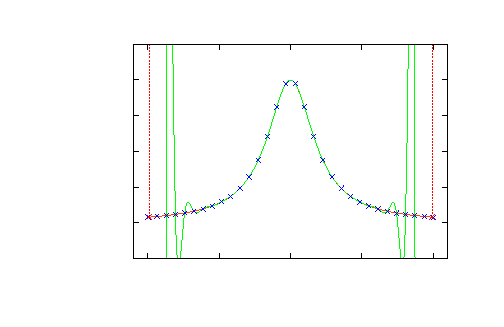
\includegraphics{32-eq}}%
    \gplfronttext
  \end{picture}%
\endgroup
% GNUPLOT: LaTeX picture with Postscript
\begingroup
  \makeatletter
  \providecommand\color[2][]{%
    \GenericError{(gnuplot) \space\space\space\@spaces}{%
      Package color not loaded in conjunction with
      terminal option `colourtext'%
    }{See the gnuplot documentation for explanation.%
    }{Either use 'blacktext' in gnuplot or load the package
      color.sty in LaTeX.}%
    \renewcommand\color[2][]{}%
  }%
  \providecommand\includegraphics[2][]{%
    \GenericError{(gnuplot) \space\space\space\@spaces}{%
      Package graphicx or graphics not loaded%
    }{See the gnuplot documentation for explanation.%
    }{The gnuplot epslatex terminal needs graphicx.sty or graphics.sty.}%
    \renewcommand\includegraphics[2][]{}%
  }%
  \providecommand\rotatebox[2]{#2}%
  \@ifundefined{ifGPcolor}{%
    \newif\ifGPcolor
    \GPcolortrue
  }{}%
  \@ifundefined{ifGPblacktext}{%
    \newif\ifGPblacktext
    \GPblacktextfalse
  }{}%
  % define a \g@addto@macro without @ in the name:
  \let\gplgaddtomacro\g@addto@macro
  % define empty templates for all commands taking text:
  \gdef\gplbacktext{}%
  \gdef\gplfronttext{}%
  \makeatother
  \ifGPblacktext
    % no textcolor at all
    \def\colorrgb#1{}%
    \def\colorgray#1{}%
  \else
    % gray or color?
    \ifGPcolor
      \def\colorrgb#1{\color[rgb]{#1}}%
      \def\colorgray#1{\color[gray]{#1}}%
      \expandafter\def\csname LTw\endcsname{\color{white}}%
      \expandafter\def\csname LTb\endcsname{\color{black}}%
      \expandafter\def\csname LTa\endcsname{\color{black}}%
      \expandafter\def\csname LT0\endcsname{\color[rgb]{1,0,0}}%
      \expandafter\def\csname LT1\endcsname{\color[rgb]{0,1,0}}%
      \expandafter\def\csname LT2\endcsname{\color[rgb]{0,0,1}}%
      \expandafter\def\csname LT3\endcsname{\color[rgb]{1,0,1}}%
      \expandafter\def\csname LT4\endcsname{\color[rgb]{0,1,1}}%
      \expandafter\def\csname LT5\endcsname{\color[rgb]{1,1,0}}%
      \expandafter\def\csname LT6\endcsname{\color[rgb]{0,0,0}}%
      \expandafter\def\csname LT7\endcsname{\color[rgb]{1,0.3,0}}%
      \expandafter\def\csname LT8\endcsname{\color[rgb]{0.5,0.5,0.5}}%
    \else
      % gray
      \def\colorrgb#1{\color{black}}%
      \def\colorgray#1{\color[gray]{#1}}%
      \expandafter\def\csname LTw\endcsname{\color{white}}%
      \expandafter\def\csname LTb\endcsname{\color{black}}%
      \expandafter\def\csname LTa\endcsname{\color{black}}%
      \expandafter\def\csname LT0\endcsname{\color{black}}%
      \expandafter\def\csname LT1\endcsname{\color{black}}%
      \expandafter\def\csname LT2\endcsname{\color{black}}%
      \expandafter\def\csname LT3\endcsname{\color{black}}%
      \expandafter\def\csname LT4\endcsname{\color{black}}%
      \expandafter\def\csname LT5\endcsname{\color{black}}%
      \expandafter\def\csname LT6\endcsname{\color{black}}%
      \expandafter\def\csname LT7\endcsname{\color{black}}%
      \expandafter\def\csname LT8\endcsname{\color{black}}%
    \fi
  \fi
    \setlength{\unitlength}{0.0500bp}%
    \ifx\gptboxheight\undefined%
      \newlength{\gptboxheight}%
      \newlength{\gptboxwidth}%
      \newsavebox{\gptboxtext}%
    \fi%
    \setlength{\fboxrule}{0.5pt}%
    \setlength{\fboxsep}{1pt}%
\begin{picture}(4534.00,2834.00)%
    \gplgaddtomacro\gplbacktext{%
      \csname LTb\endcsname%%
      \put(990,499){\makebox(0,0)[r]{\strut{}\num{-0.25}}}%
      \put(990,842){\makebox(0,0)[r]{\strut{}\num{0}}}%
      \put(990,1184){\makebox(0,0)[r]{\strut{}\num{0.25}}}%
      \put(990,1527){\makebox(0,0)[r]{\strut{}\num{0.5}}}%
      \put(990,1869){\makebox(0,0)[r]{\strut{}\num{0.75}}}%
      \put(990,2212){\makebox(0,0)[r]{\strut{}\num{1}}}%
      \put(990,2554){\makebox(0,0)[r]{\strut{}\num{1.25}}}%
      \put(1259,279){\makebox(0,0){\strut{}\num{-1}}}%
      \put(1944,279){\makebox(0,0){\strut{}\num{-0.5}}}%
      \put(2630,279){\makebox(0,0){\strut{}\num{0}}}%
      \put(3315,279){\makebox(0,0){\strut{}\num{0.5}}}%
      \put(4000,279){\makebox(0,0){\strut{}\num{1}}}%
      \put(2355,855){\makebox(0,0)[l]{\strut{}$ n = 32 $}}%
    }%
    \gplgaddtomacro\gplfronttext{%
    }%
    \gplbacktext
    \put(0,0){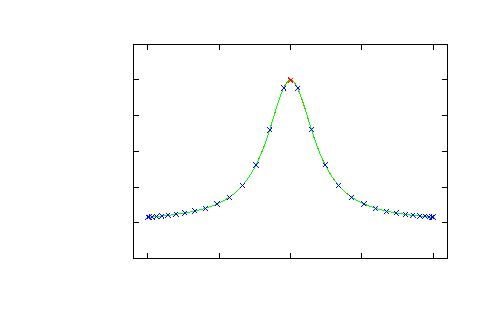
\includegraphics{32-cheb}}%
    \gplfronttext
  \end{picture}%
\endgroup

	\caption{Resultat d'interpolar \( f \) fent servir \( n \) nodes equidistants (esquerra) i \( n \) nodes de Chebyshev (dreta). En vermell s'indica el màxim error comès.}
	\label{fig:interpolacio}
\end{figure}

\newpage

\section{Problema 2}
Considerem la funció de Bessel de primera espècie d'ordre zero, $J_0(x)$. Volem estimar els valors de les arrels de \( J_0 \), és a dir, de les \( x^{\ast} \) tals que \( J_0(x^{\ast}) = 0 \). Una manera de fer-ho és interpolar la inversa de \( J_0 \) a l'interval \( (1.9, 3) \). En aquest interval \( J_0 \) és localment invertible ja que és estrictament decreixent i derivable. Concretament construirem el polinomi interpolador que té per nodes \( (J_0(x_n), x_n) \). D'aquesta manera, si \( p \) és el polinomi que obtenim, \( p(0) \) és una aproximació de \( x^{\ast} \).

La tria de nodes s'ha fet de tres maneres diferents. En primer lloc s'ha interpolat a partir dels nodes amb valors de \( J_0(x) \) positius i més propers al canvi de signe. Similarment s'ha interpolat a partir dels nodes amb \( J_0(x) \) negatiu i més proper al canvi de signe. I per últim s'ha interpolat prenent un nombre igual de nodes amb \( J_0(x) \) positiu i negatiu al voltant del canvi de signe.    

El programa \texttt{prob2.c} calcula el polinomi interpolador de Lagrange amb el mètode de les diferències dividides de Newton a partir d'un conjunt de nodes donats. Seguidament l'avalua a \( x=0 \) fent servir la regla de Horner. La interpolació s'ha fet de grau 1, 3 i 5 --és a dir , amb 2, 4, i 6 nodes--- seguint cada un dels tres mètodes detallats anteriorment. Els resultats es mostren a les \cref{tab:Bessel positius,tab:Bessel negatius,tab:Bessel simetrics}, on també es mostra el resultat d'avaluar \( J_0 \) a l'aproximació de l'arrel per tenir una idea de com de bones són cada aproximació ---evidentment, com més proper a 0 és \( J_0(x^{\ast}) \), millor és l'aproximació---. 

\begin{table}[htb]
	\sffamily \small	\centering
	\caption{Aproximació de l'arrel de \( J_0 \) interpolant a partir de nodes positius propers al canvi de signe. }	
	\label{tab:Bessel positius}
	\begin{tabular}{cS[table-parse-only]S[table-parse-only]}
		\toprule
		{Grau} & { \( x^{\ast} \) } & { \( J_0(x^{\ast}) \) } \\
		\midrule
		1 & 2.404728613882804 & 5.03291522479392d-5\\
		3 & 2.404822718113948 & 1.47416266795862d-6\\
		5 & 2.404825294785460 & 1.36489238329446d-7\\
		\bottomrule
	\end{tabular}
\end{table}

\begin{table}[htb]
	\sffamily \small	\centering
	\caption{Aproximació de l'arrel de \( J_0 \) interpolant a partir de nodes negatius propers al canvi de signe. }	
	\label{tab:Bessel negatius}
	\begin{tabular}{cS[table-parse-only]S[table-parse-only]}
		\toprule
		{Grau} & { \( x^{\ast} \) } & { \( J_0(x^{\ast}) \) } \\
		\midrule
		1 & 2.400077241947102 & 2.46750381340249d-3\\
		3 & 2.404149375353531 & 3.51087705194527d-4\\
		5 & 2.404216734868258 & 3.16108843546827d-4\\
		\bottomrule
	\end{tabular}
\end{table}

\begin{table}[htb]
	\sffamily \small	\centering
	\caption{Aproximació de l'arrel de \( J_0 \) interpolant a partir de nodes simètrics al voltant del canvi de signe. }	
	\label{tab:Bessel simetrics}
	\begin{tabular}{cS[table-parse-only]S[table-parse-only]}
		\toprule
		{Grau} & { \( x^{\ast} \) } & { \( J_0(x^{\ast}) \) } \\
		\midrule
		1 & 2.404927513002775 & -5.29287203952310d-5\\
		3 & 2.404824021911155 & 7.97298995297100d-8\\
		5 & 2.404825653043717 & -4.94996456864148d-8\\
		\bottomrule
	\end{tabular}
\end{table}

El millor resultat l'obtenim amb la interpolació de grau 5 a partir de valors simètrics al voltant del canvi de signe de $J_0$. En general les millors són les interpolacions amb els valors positius i amb els simètrics, i la interpolació amb valors negatius és prou dolenta en comparació.

De fet ja podiem esperar des del principi que la millor interpolació fos la simètrica, ja que és l'única que conté l'arrel a l'envolupant convexa dels nodes. A més, en general si tenim els nodes d'interpolació continguts en un interval $[a,b]$ i volem avaluar el polinomi interpolador $p(x)$ en un punt fora d'aquest interval l'error obtingut pot ser molt gran.

\newpage

\section{Problema 3}
El nostre objectiu és obtenir un valor aproximat de la integral
\begin{equation}\label{eq:integral 3}
	I=\int^{1}_0\dfrac{dx}{1+x^2} = \arctan(1) - \arctan(0) = \frac{1}{4}\pi \approx \num{0.785398163397448}
\end{equation}
pel mètode dels trapezis i pel mètode de Simpson dividint l'interval $[0,1]$ en quatre parts iguals.

El programa \texttt{prob3.c} calcula aquestes aproximacions així com una fita de l'error que es comet amb cadascuna. Fent servir el mètode dels trapezis hem obtingut $I \approx \num{0.782794117647059}$, que comparat amb el valor exacte fins a $15$ decimals de l'\cref{eq:integral 3} ens dóna un error aproximat de $\num{2.604045750389d-3}$.
Amb el mètode de Simpson obtenim $I \approx \num{0.785392156862745}$, que comparat amb l'\cref{eq:integral 3} té un error aproximat de $\num{6.006534703d-6}$.

Per tant veiem que amb la regla de Simpson hem obtingut una millor aproximació.

\newpage

\section{Problema 4}
Volem obtenir un valor aproximat de la integral
\begin{equation*}
	I=\int^{5}_1 \dfrac{e^x}{x} \,dx
\end{equation*}
pel mètode dels trapezis dividint l'interval $[1,5]$ en 4, 8, 16, 32 i 64 parts iguals.

El programa \texttt{prob4.c} calcula aquestes aproximacions i una estimació de l'error comés. Els resultats obtinguts per a cada $n$ es mostren a la \cref{tab:resultats 4}. 

\begin{table}[h]
	\centering \sffamily \small
	\caption{Resultat i estimació de l'error obtingut per a cada \( n \).}	
	\label{tab:resultats 4}
	\begin{tabular}{cS[table-parse-only]S[table-parse-only]}
		\toprule
		{ \( n \) } & {Aproximació de \( I \) } & { Estimació de l'error } \\
		\midrule
		4 & 40.239701356634455 & 10\\
		8 & 38.782928156314796 & 2.5\\
		16 & 38.413711363539406 & 0.625\\
		32 & 38.321069162332130 & 0.15625\\
		64 & 38.297886904128802 & 0.0390625\\
		\bottomrule
	\end{tabular}
\end{table}

L'estimació de l'error l'hem calculat segons la fórmula:
\begin{equation*}
	\abs{\dfrac{(b-a)F}{12}h^2},
\end{equation*}
on $b$ i $a$ són els extrems de l'interval ---en el nostre cas $b=5$ i $a=1$---, $F$ és una fita superior en l'interval de la segona derivada de la funció que volem integrar, i $h=(b-a)/n$ amb \( n \) el nombre de parts en les que dividim l'interval. Tenim, per tot \( x \geqslant 1 \) 
\begin{equation*}
	\frac{d^2}{dx^2}\left(\frac{e^x}{x}\right) = \dfrac{e^x(x^3-2x^2+2x)}{x^4} \leqslant \dfrac{e^x}{x},
\end{equation*}
per tant, com que \( e^{x}/x \) és creixent a l'interval \( [1,5] \) podem fitar la segona derivada per $F=e^5/5 \leqslant 30$. De manera que per a cada $n$ ens queda que l'error està fitat per \( 160  n^{-2} \). Observem que per a un major nombre de divisions del interval esperem millorar l'aproximació de $I$.

\newpage

\section{Problema 5}
Volem calcular amb un error menor que $10^{-2}$ el valor de la integral
\begin{equation*}
	I = \int_{1}^{2}\log(x) \, dx
\end{equation*}
utilitzant la regla composta de Simpson.

Una fita de l'error amb aquest mètode ve donada per
\begin{equation*}
	\varepsilon = \abs{\dfrac{(b-a)F}{180}h^4 } 
\end{equation*}
on $b$, $a$ són els extrems del interval, $F$ és una fita superior del valor absolut de la quarta derivada de la funció que volem integrar, i $h=(b-a)/n$ on $n$ és el nombre de divisions de l'interval. En el nostre cas $a=1$, $b=2$, $|f^{(4)}(x)|=|-6/x^4|\leqslant 6$ per a $x\in[1,2]$, de manera que volem
\begin{equation*}
	\abs{\frac{6}{180} \dfrac{1}{n^4}} \leqslant 10^{-2} 
\end{equation*}
Per tant necessitarem fer com a mínim $n=2$ divisions de l'interval $[1,2]$ per obtenir la precisió demanada.

El programa \texttt{prob5.c} calcula aquesta integral amb diversos valors de $n$. Els resultats es mostren a la \cref{tab:resultats 5}.
\begin{table}[htb]
	\centering \small \sffamily
	\caption{Resultats per a diversos $n$ parells}	
	\label{tab:resultats 5}
	\begin{tabular}{cS[table-parse-only]}
		\toprule
		{ \( n \) } & {Aproximació de \( I \) } \\
		\midrule
		2 & 0.385834602165434 \\
		4 & 0.386259562814567 \\
		6 & 0.386287163278802 \\
		8 & 0.386292043466313 \\
		10 & 0.386293403804806 \\
		12 & 0.386293897301413 \\
		14 & 0.386294110052020 \\
		16 & 0.386294213675793 \\
		18 & 0.386294268953807 \\
		20 & 0.386294300594357 \\
		\bottomrule
	\end{tabular}
\end{table}

Observem que amb $n=2$ iteracions ja hem obtingut dues xifres decimals correctes, per tant la nostra estimació de l'error ha sigut adequada. Si volem garantir un error menor que $10^{-4}$ necessitem $n \geqslant \ceil[\Big]{\sqrt[4]{10^4/30}\,} = 19$ i com que $n$ ha de ser parell $n=20$.

\newpage

\section{Problema 6}
En aquest problema se'ns demana de calcular una aproximació de la distància recorreguda per un automòbil a partir d'un conjunt finit de valors de la seva velocitat a certs instants de temps. En concret volem aproximar la integral
\begin{equation*}
	L=\int_{0}^{84}v(t) \, dt,
\end{equation*}
tenint només valors de \( v(t) \) cada \SI{6}{s}. Per tant estem dividint l'interval $[0,84]$ en $n=14$ parts iguals. Per a trobar $L$ utilitzarem la regla de Simpson composta, ja que en general dóna un millor resultat que la regla dels trapezis composta. 

El programa \texttt{prob6.c} calcula aquesta aproximació. El resultat que obtenim és \( L = \SI{2909.400000000000091}{m} \), per tant la pista mesura aproximadament \SI{2.909}{km}.

\newpage
\section{Problema 7}
\begin{figure}[b]
	\centering
	\sffamily \footnotesize
	% GNUPLOT: LaTeX picture with Postscript
\begingroup
  \makeatletter
  \providecommand\color[2][]{%
    \GenericError{(gnuplot) \space\space\space\@spaces}{%
      Package color not loaded in conjunction with
      terminal option `colourtext'%
    }{See the gnuplot documentation for explanation.%
    }{Either use 'blacktext' in gnuplot or load the package
      color.sty in LaTeX.}%
    \renewcommand\color[2][]{}%
  }%
  \providecommand\includegraphics[2][]{%
    \GenericError{(gnuplot) \space\space\space\@spaces}{%
      Package graphicx or graphics not loaded%
    }{See the gnuplot documentation for explanation.%
    }{The gnuplot epslatex terminal needs graphicx.sty or graphics.sty.}%
    \renewcommand\includegraphics[2][]{}%
  }%
  \providecommand\rotatebox[2]{#2}%
  \@ifundefined{ifGPcolor}{%
    \newif\ifGPcolor
    \GPcolortrue
  }{}%
  \@ifundefined{ifGPblacktext}{%
    \newif\ifGPblacktext
    \GPblacktextfalse
  }{}%
  % define a \g@addto@macro without @ in the name:
  \let\gplgaddtomacro\g@addto@macro
  % define empty templates for all commands taking text:
  \gdef\gplbacktext{}%
  \gdef\gplfronttext{}%
  \makeatother
  \ifGPblacktext
    % no textcolor at all
    \def\colorrgb#1{}%
    \def\colorgray#1{}%
  \else
    % gray or color?
    \ifGPcolor
      \def\colorrgb#1{\color[rgb]{#1}}%
      \def\colorgray#1{\color[gray]{#1}}%
      \expandafter\def\csname LTw\endcsname{\color{white}}%
      \expandafter\def\csname LTb\endcsname{\color{black}}%
      \expandafter\def\csname LTa\endcsname{\color{black}}%
      \expandafter\def\csname LT0\endcsname{\color[rgb]{1,0,0}}%
      \expandafter\def\csname LT1\endcsname{\color[rgb]{0,1,0}}%
      \expandafter\def\csname LT2\endcsname{\color[rgb]{0,0,1}}%
      \expandafter\def\csname LT3\endcsname{\color[rgb]{1,0,1}}%
      \expandafter\def\csname LT4\endcsname{\color[rgb]{0,1,1}}%
      \expandafter\def\csname LT5\endcsname{\color[rgb]{1,1,0}}%
      \expandafter\def\csname LT6\endcsname{\color[rgb]{0,0,0}}%
      \expandafter\def\csname LT7\endcsname{\color[rgb]{1,0.3,0}}%
      \expandafter\def\csname LT8\endcsname{\color[rgb]{0.5,0.5,0.5}}%
    \else
      % gray
      \def\colorrgb#1{\color{black}}%
      \def\colorgray#1{\color[gray]{#1}}%
      \expandafter\def\csname LTw\endcsname{\color{white}}%
      \expandafter\def\csname LTb\endcsname{\color{black}}%
      \expandafter\def\csname LTa\endcsname{\color{black}}%
      \expandafter\def\csname LT0\endcsname{\color{black}}%
      \expandafter\def\csname LT1\endcsname{\color{black}}%
      \expandafter\def\csname LT2\endcsname{\color{black}}%
      \expandafter\def\csname LT3\endcsname{\color{black}}%
      \expandafter\def\csname LT4\endcsname{\color{black}}%
      \expandafter\def\csname LT5\endcsname{\color{black}}%
      \expandafter\def\csname LT6\endcsname{\color{black}}%
      \expandafter\def\csname LT7\endcsname{\color{black}}%
      \expandafter\def\csname LT8\endcsname{\color{black}}%
    \fi
  \fi
    \setlength{\unitlength}{0.0500bp}%
    \ifx\gptboxheight\undefined%
      \newlength{\gptboxheight}%
      \newlength{\gptboxwidth}%
      \newsavebox{\gptboxtext}%
    \fi%
    \setlength{\fboxrule}{0.5pt}%
    \setlength{\fboxsep}{1pt}%
\begin{picture}(4534.00,2834.00)%
    \gplgaddtomacro\gplbacktext{%
      \csname LTb\endcsname%%
      \put(990,499){\makebox(0,0)[r]{\strut{}\num{-0.25}}}%
      \put(990,842){\makebox(0,0)[r]{\strut{}\num{0}}}%
      \put(990,1184){\makebox(0,0)[r]{\strut{}\num{0.25}}}%
      \put(990,1527){\makebox(0,0)[r]{\strut{}\num{0.5}}}%
      \put(990,1869){\makebox(0,0)[r]{\strut{}\num{0.75}}}%
      \put(990,2212){\makebox(0,0)[r]{\strut{}\num{1}}}%
      \put(990,2554){\makebox(0,0)[r]{\strut{}\num{1.25}}}%
      \put(1259,279){\makebox(0,0){\strut{}\num{-1}}}%
      \put(1944,279){\makebox(0,0){\strut{}\num{-0.5}}}%
      \put(2630,279){\makebox(0,0){\strut{}\num{0}}}%
      \put(3315,279){\makebox(0,0){\strut{}\num{0.5}}}%
      \put(4000,279){\makebox(0,0){\strut{}\num{1}}}%
      \put(2355,855){\makebox(0,0)[l]{\strut{}$ n = 4 $}}%
    }%
    \gplgaddtomacro\gplfronttext{%
    }%
    \gplbacktext
    \put(0,0){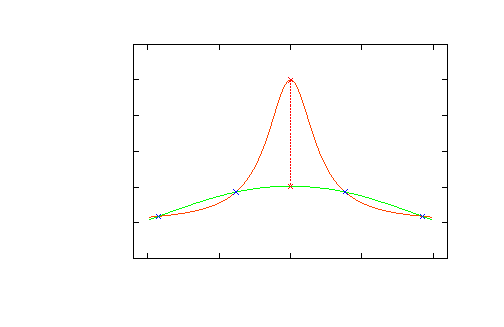
\includegraphics{04-splines}}%
    \gplfronttext
  \end{picture}%
\endgroup
% GNUPLOT: LaTeX picture with Postscript
\begingroup
  \makeatletter
  \providecommand\color[2][]{%
    \GenericError{(gnuplot) \space\space\space\@spaces}{%
      Package color not loaded in conjunction with
      terminal option `colourtext'%
    }{See the gnuplot documentation for explanation.%
    }{Either use 'blacktext' in gnuplot or load the package
      color.sty in LaTeX.}%
    \renewcommand\color[2][]{}%
  }%
  \providecommand\includegraphics[2][]{%
    \GenericError{(gnuplot) \space\space\space\@spaces}{%
      Package graphicx or graphics not loaded%
    }{See the gnuplot documentation for explanation.%
    }{The gnuplot epslatex terminal needs graphicx.sty or graphics.sty.}%
    \renewcommand\includegraphics[2][]{}%
  }%
  \providecommand\rotatebox[2]{#2}%
  \@ifundefined{ifGPcolor}{%
    \newif\ifGPcolor
    \GPcolortrue
  }{}%
  \@ifundefined{ifGPblacktext}{%
    \newif\ifGPblacktext
    \GPblacktextfalse
  }{}%
  % define a \g@addto@macro without @ in the name:
  \let\gplgaddtomacro\g@addto@macro
  % define empty templates for all commands taking text:
  \gdef\gplbacktext{}%
  \gdef\gplfronttext{}%
  \makeatother
  \ifGPblacktext
    % no textcolor at all
    \def\colorrgb#1{}%
    \def\colorgray#1{}%
  \else
    % gray or color?
    \ifGPcolor
      \def\colorrgb#1{\color[rgb]{#1}}%
      \def\colorgray#1{\color[gray]{#1}}%
      \expandafter\def\csname LTw\endcsname{\color{white}}%
      \expandafter\def\csname LTb\endcsname{\color{black}}%
      \expandafter\def\csname LTa\endcsname{\color{black}}%
      \expandafter\def\csname LT0\endcsname{\color[rgb]{1,0,0}}%
      \expandafter\def\csname LT1\endcsname{\color[rgb]{0,1,0}}%
      \expandafter\def\csname LT2\endcsname{\color[rgb]{0,0,1}}%
      \expandafter\def\csname LT3\endcsname{\color[rgb]{1,0,1}}%
      \expandafter\def\csname LT4\endcsname{\color[rgb]{0,1,1}}%
      \expandafter\def\csname LT5\endcsname{\color[rgb]{1,1,0}}%
      \expandafter\def\csname LT6\endcsname{\color[rgb]{0,0,0}}%
      \expandafter\def\csname LT7\endcsname{\color[rgb]{1,0.3,0}}%
      \expandafter\def\csname LT8\endcsname{\color[rgb]{0.5,0.5,0.5}}%
    \else
      % gray
      \def\colorrgb#1{\color{black}}%
      \def\colorgray#1{\color[gray]{#1}}%
      \expandafter\def\csname LTw\endcsname{\color{white}}%
      \expandafter\def\csname LTb\endcsname{\color{black}}%
      \expandafter\def\csname LTa\endcsname{\color{black}}%
      \expandafter\def\csname LT0\endcsname{\color{black}}%
      \expandafter\def\csname LT1\endcsname{\color{black}}%
      \expandafter\def\csname LT2\endcsname{\color{black}}%
      \expandafter\def\csname LT3\endcsname{\color{black}}%
      \expandafter\def\csname LT4\endcsname{\color{black}}%
      \expandafter\def\csname LT5\endcsname{\color{black}}%
      \expandafter\def\csname LT6\endcsname{\color{black}}%
      \expandafter\def\csname LT7\endcsname{\color{black}}%
      \expandafter\def\csname LT8\endcsname{\color{black}}%
    \fi
  \fi
    \setlength{\unitlength}{0.0500bp}%
    \ifx\gptboxheight\undefined%
      \newlength{\gptboxheight}%
      \newlength{\gptboxwidth}%
      \newsavebox{\gptboxtext}%
    \fi%
    \setlength{\fboxrule}{0.5pt}%
    \setlength{\fboxsep}{1pt}%
\begin{picture}(4534.00,2834.00)%
    \gplgaddtomacro\gplbacktext{%
      \csname LTb\endcsname%%
      \put(990,499){\makebox(0,0)[r]{\strut{}\num{-0.25}}}%
      \put(990,842){\makebox(0,0)[r]{\strut{}\num{0}}}%
      \put(990,1184){\makebox(0,0)[r]{\strut{}\num{0.25}}}%
      \put(990,1527){\makebox(0,0)[r]{\strut{}\num{0.5}}}%
      \put(990,1869){\makebox(0,0)[r]{\strut{}\num{0.75}}}%
      \put(990,2212){\makebox(0,0)[r]{\strut{}\num{1}}}%
      \put(990,2554){\makebox(0,0)[r]{\strut{}\num{1.25}}}%
      \put(1259,279){\makebox(0,0){\strut{}\num{-1}}}%
      \put(1944,279){\makebox(0,0){\strut{}\num{-0.5}}}%
      \put(2630,279){\makebox(0,0){\strut{}\num{0}}}%
      \put(3315,279){\makebox(0,0){\strut{}\num{0.5}}}%
      \put(4000,279){\makebox(0,0){\strut{}\num{1}}}%
      \put(2355,855){\makebox(0,0)[l]{\strut{}$ n = 4 $}}%
    }%
    \gplgaddtomacro\gplfronttext{%
    }%
    \gplbacktext
    \put(0,0){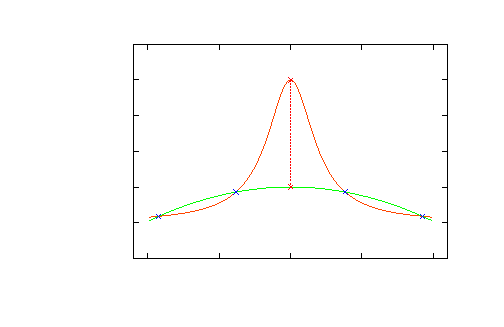
\includegraphics{04-cheb}}%
    \gplfronttext
  \end{picture}%
\endgroup

	\caption{Resultat d'interpolar \( f \) fent servir interpolació per splines cúbics amb quatre nodes (esquerra) i 4 nodes de Chebyshev (dreta). En vermell s'indica el màxim error comès.}
	\label{fig:splines}	
\end{figure}

Una altra manera d'interpolar funcions que és més estable quan el nombre de nodes creix és a partir de splines. En lloc de construir un polinomi de grau molt alt es construeixen molts polinomis de grau baix ---els splines solen ser cúbics--- imposant condicions de regularitat als nodes. Concretament hem fet servir splines cúbics amb condicions d'extrem naturals, és a dir, imposant
\begin{equation*}
	s_0''(x_0) = s_n''(x_n) = 0,
\end{equation*}
on denotarem per \( s_i \) l'spline \( i \)-èssim. Podem escriure
\begin{equation*}
	s_i = a_{i0} + a_{i1}(x-x_i) + a_{i2}(x-x)^2 + a_{i3}(x-x_i)^3.
\end{equation*}
Per tant hem de calcular els coeficients \( a_{ij} \). La manera estàndard de procedir és considerar els anomenats moments, \( M_i \defeq s_i''(x_i) \), que són la solució d'un sistema lineal que només involucra els nodes d'interpolació \( \{(x_i,f(x_i)\} \). A partir dels moments podem reconstruir la resta de coeficients com
\begin{equation} \label{eq:coeficients splines}
	\begin{aligned}
		a_{i0} & = f(x_i) \\
		a_{i1} & = \frac{f(x_{i+1}) - f(x_i)}{x_{i+1} - x_i} - \frac{2M_{i+1} + M_i}{6}(x_{i+1} - x_i) \\
		a_{i2} & = \frac{M_i}{2} \\
		a_{i3} & = \frac{M_{i+1} - M_i}{6(x_{i+1} - x_i)}
	\end{aligned} 
\end{equation}

\parbreak

Per aproximar \( f \) definida com al problema \ref{sec:Problema 1} amb quatre splines cúbics primer hem resolt el sistema que determina els moments fent servir 4 nodes de Chebyshev mitjançant \textsf{SageMath} i hem obtingut 
\begin{equation*}
	\begin{aligned}
		M_0 = M_3 &= 0 \\
		M_1 = M_2 &= \num{-0.557114}.
	\end{aligned}
\end{equation*}
El programa \texttt{prob7.c} llegeix la llista de nodes i de moments i implementa els càlculs de l'\cref{eq:coeficients splines}. Fet això, avalua els splines als 181 punts proposats al problema \ref{sec:Problema 1} i busca l'error màxim comès a la interpolació. El resultat, així com la mateixa interpolació fent servir diferències dividides amb quatre nodes de Chebyshev es mostra a la \cref{fig:splines}. 

Tal i com podem apreciar, la diferència entre ambdós mètodes és petita. En part és perquè 4 és un nombre més aviat petit de nodes, a partir dels quals es pot extreure poca informació sobre la funció a interpolar. En particular, en aquest cas no estem donant pràcticament cap tipus d'informació sobre el comportament de \( f \) al voltant del 0. Per a realitzar la interpolació amb un nombre arbitrari d'splines caldria un programa que resolvés el sistema que determina els moments, per al qual encara no disposem d'eines. Així doncs no hem pogut fer la interpolació amb splines per a nombres elevats de nodes. Tot i així és raonable concloure que fer servir diferències dividides amb els nodes de Chebyshev és molt més eficient que no pas fer servir splines, ja que no involucra la resolució d'un sistema i només requereix de \( n+1 \) coeficients, en contra dels \( 4(n - 1) \) coeficients necessaris pels splines.

\end{document}
